% In this section we describe the data used to train \system.

% \iffalse
% The continual pretraining process followed a carefully designed two-stage curriculum.  The first stage included a big corpus of general multilingual web data. This extensive training aimed to expose the model to a diverse range of data and establish a strong foundation for the subsequent stage. In the second stage, we employed a strategic data mixing approach to enhance the model's performance in specific areas and align it with our desired objectives. Following \cite{taylor2022galactica, Li2021Colossal}, we also mixed in publicly available instruction tuning datasets in both stages of training.

% The first stage contains 377B tokens of processed and filtered web data from the Stack, RefinedWeb~\citep{refinedweb}, RedPajama~\citep{together2023redpajama} and the Pile~\citep{gao2020pile} along with a multilingual dataset that we created, containing text in Japanese, English, Vietnamese, Hindi and Finnish. For the distribution of languages, please see Figure \ref{fig:distribution}. We also mix in lower quality instruction tuning datasets during this stage of training.

% For the second stage, we chose to use an expanded mix of high quality instructions, code, reasoning and domain-specific datasets. The latter was included for the purpose of future work on expert models \citep{li2022branchtrainmerge, feng2024mixtureofloras}. Additionally, we included a safety instructions dataset called BidenHarrisRedteam, which is described in section \ref{bidenharris}. For the full list of datasets, please see Appendix \ref{datasets}. The total data size for this stage is 58B tokens.
% \fi

%We curated and cleaned a 435B token dataset, 377B of which was used for the first stage of training, and the remaining 58B tokens for the second stage. 

\paragraph{Data Curation.} The continual pretraining process for training \system\ followed a carefully designed two-stage curriculum, as shown in Fig.~\ref{fig:distribution}.
In the first stage, termed as \textbf{Continual Auxiliary Pretraining} (CAP), a large corpus of general multilingual web data was used to expose the model to diverse data, laying a robust foundation for subsequent training. The second stage, termed as \textbf{Continual Alignment Tuning} (CAT) employed a strategic data-mixing approach to bolster the model's performance in targeted areas and align it with our predefined objectives. Following \citet{taylor2022galactica} and \citet{Li2021Colossal}, we also included publicly available instruction tuning datasets in both stages of training. 

%Our continual pretraining dataset comprises a diverse mixture of multilingual, code and instruction data. %By mixing in instructions during continued pretraining, we could evaluate our model's performance on instruction following at different checkpoints. 

% In the first training stage dataset, we included 435B tokens of processed and filtered web data from the Stack~\citep{kocetkov2022stack}, RefinedWeb~\citep{refinedweb}, RedPajama~\citep{together2023redpajama} and the Pile~\citep{gao2020pile} (other than Pile-CC) along with multilingual data from HPLT~\citep{degibert2024new}, MC4~\citep{zhu2023multimodal}, Paracrawl~\citep{ghussin2023exploring}, OSCAR~\citep{abadji2022cleaner}, Wikipedia~\citep{wikidump} and instruction tuning data including from OpenAssistant~\citep{kopf2023openassistant}, APIBench~\citep{patil2023gorilla} and OIG~\citep{oig2023}. 

In CAP, we incorporated 377B tokens of processed and filtered web data from various sources, including Stack~\citep{kocetkov2022stack}, RefinedWeb~\citep{refinedweb}, RedPajama~\citep{together2023redpajama}, and a subset of the Pile~\citep{gao2020pile}. Additionally, multilingual data from HPLT~\citep{degibert2024new}, MC4~\citep{zhu2023multimodal}, Paracrawl~\citep{ghussin2023exploring}, OSCAR~\citep{abadji2022cleaner}, along with Wikipedia~\citep{wikidump}, and instruction tuning data from sources such as OpenAssistant~\citep{kopf2023openassistant}, APIBench~\citep{patil2023gorilla}, and OIG~\citep{oig2023} were included. 


For CAT, we opted for a greater percentage of code and a changed mix of high-quality public instruction datasets \citep{mishra2022crosstask, ding2023enhancing, ivison2023camels}, encompassing coding \citep{luo2023wizardcoder, mishra2023prompting} and mathematical reasoning \citep{yu2023metamath, mishra2023lila}. The intention was to not overfit to the high quality instruction data, and thus the high quality data was used in CAT only.  We also subsampled data from CAP for quality, as described below. Furthermore, we introduced a new safety instruction dataset named \textbf{Biden-Harris Redteam}, detailed in Section \ref{sec:safety}. The total dataset size for CAT is 58B tokens.
% 
We refer the reader to Fig. \ref{fig:distribution} for the distribution of languages in both training stages. The complete list of datasets is available in Appendix \ref{datasets}.

\begin{figure}[t]
\centering
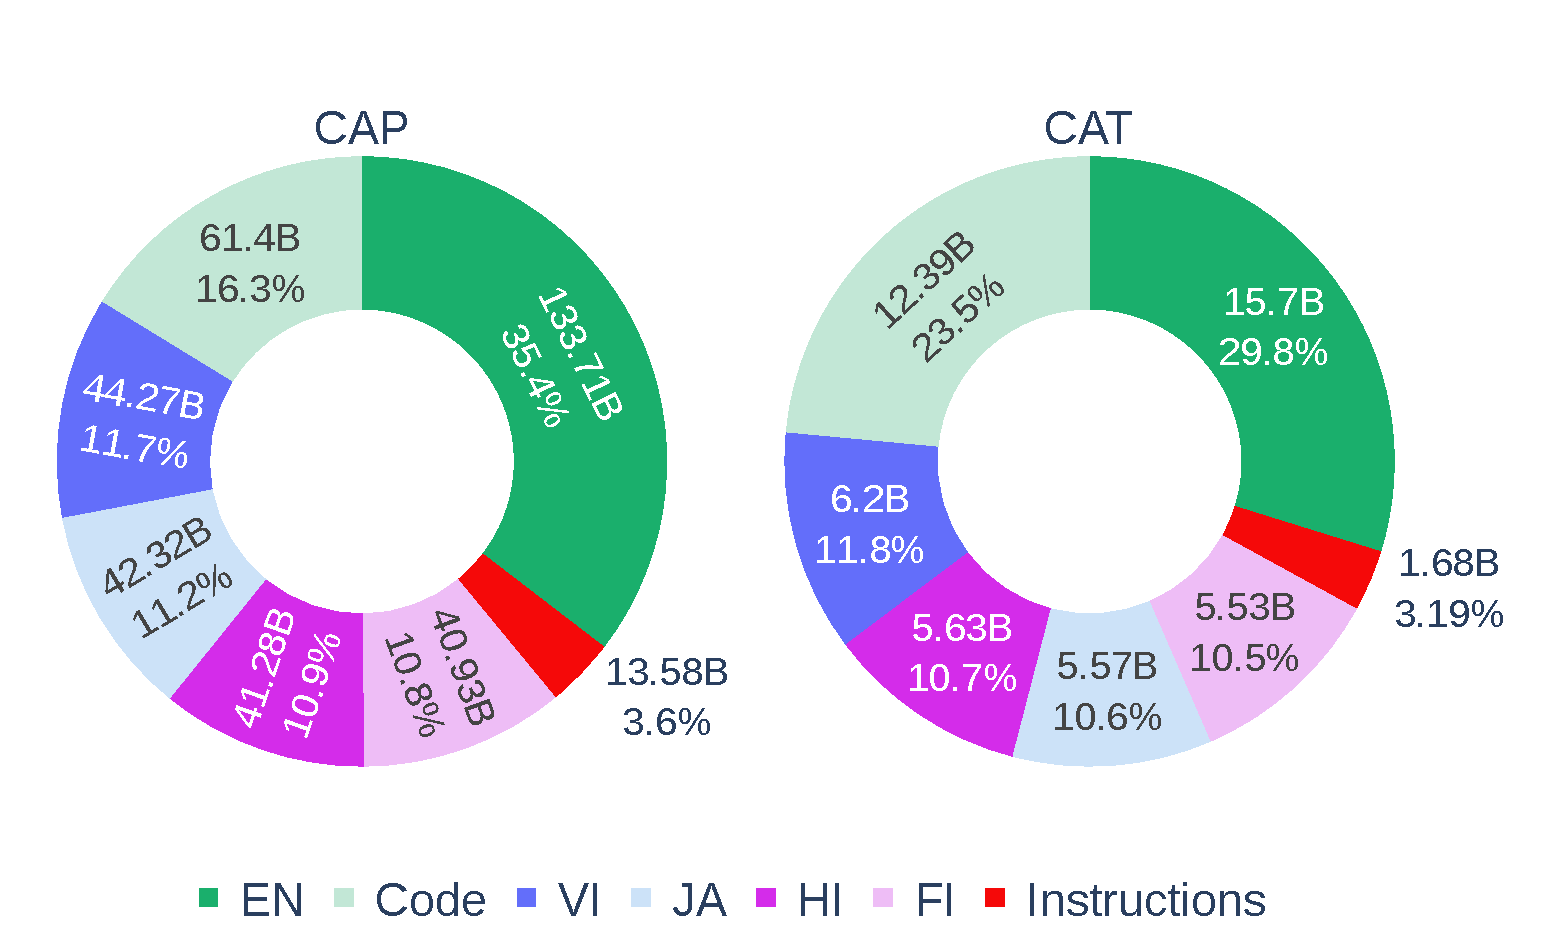
\includegraphics[width=\columnwidth]{fig/output_file.pdf}
\caption{Training data distribution of languages, code, and instructions used for the two-stage continual pretraining of the \system\ model. There are a total of \texttt{377B} and \texttt{58B} tokens in the Continual Auxiliary Pretraining (CAP) and Continual Alignment Tuning (CAT) stages respectively.} 
\vspace{-3mm}
\label{fig:distribution}
\end{figure}

\paragraph{Data Filtering.}
% To remove toxic content and low quality text, we used similar filters as carried out in ~\cite{nguyen2023culturax, scao2022bloom} (e.g., stop-word proportions and length of text). 

% For all web text, we followed a process similar to \cite{refinedweb} to remove low-quality content such as duplicates of headers and footers. For the second stage dataset, we further filtered web text if they had high proportions of symbols and numbers.

% For RefinedWeb, we used the RedPajama fastText classifier to retain English webpages likely to be be ``high- quality'' data similar to Wikipedia-linked articles. We trained and utilized similar classifier to filter the other languages in our dataset, aside from Finnish where the procedure resulted in over-filtering.

To remove toxic content and low-quality text, we applied filters similar to those used in~\citet{nguyen2023culturax} and \citet{scao2022bloom}, such as stop-word proportions and text length.
% 
For all web text, we followed a process akin to~\citet{refinedweb} to remove low-quality content, including duplicate headers and footers. Additionally, in the CAT dataset, we further filtered web text with high proportions of symbols and numbers.
% 
In the case of RefinedWeb~\citep{refinedweb}, we utilized the RedPajama~\citep{together2023redpajama} fastText classifier to retain English webpages resembling "high-quality" content similar to Wikipedia-linked articles. We trained and employed a similar classifier to filter other languages in our dataset, except for Finnish, where the procedure caused over-filtering, resulting in an excessively low sample volume post-filtering.
% 
% 
%We also trained and utilized similar classifiers for Japanese, Finnish, Vietnamese and Hindi \citep{touvron2023llama}. However, based on our tests, the Finnish over-filtered, so we only used the filters on the other languages. 
% 
To further enhance the quality of the RefinedWeb data, we adopted an approach detailed in \citet{ronnqvist-etal-2021-multilingual}. We trained a fastText classifier\footnote{Similar to \url{https://github.com/TurkuNLP/register-labeling?tab=readme-ov-file}} and selectively subsampled web pages with over-represented registers, aiming to retain more "rare" text (e.g., lyrical or poetic text). This filtering process was specifically applied to English text due to the prohibitive slowness of our multilingual classifiers. Addressing this limitation represents an area for future research.


%Using proportion of flagged words, we labeled a very small subset (less than 1\%) of web text with ratings to enhance control over the model. This approach follows the methodology outlined by \citet{anil2023palm}.


\paragraph{Data Processing.}
In the second stage dataset, we undertook the detection and anonymization of sensitive information, including government IDs, within web-based texts to uphold privacy and ethical standards similar to \citet{scao2022bloom}. For data segments derived from arXiv, USPTO, and StackExchange within the Pile dataset~\citep{gao2020pile}, we reconstructed the data from the original source to restore metadata, which we then appropriately appended to the texts.
 %\citep{korbak2023pretraining,anil2023palm}.
% [cite CTRL, https://arxiv.org/abs/2302.08582 and palm2]  

\iffalse
\paragraph{Data Filtering}
We used the RedPajama fastText classifier to filter out pages with low likelihood of being Wikipedia-linked articles. We trained similar classifiers for Japanese, Finnish, Vietnamese, and Hindi but found that these were less effective because Wikipedia-linked articles in those languages were much more limited.

To handle toxic content, we used similar filters as carried out in \cite{nguyen2023culturax,nguyen2024culturay,scao2022bloom}. Unlike the latter, we removed only content that is considered illegal. For other types of toxic content, we had reduced its frequency to increase the representation of other domains. Furthermore, we labeled this content with ratings to enhance control over the model. This approach follows the methodology outlined by \citet{anil2023palm}. For all web text, we followed \cite{refinedweb} to remove low-quality content such as duplicates of headers across documents, which are common on pages originating from big web publishers.

\paragraph{Data Processing}
This dataset was cleaned using standard methods similar to what was done with Cultura-X~\citep{nguyen2023culturax}. For the arXiv, USPTO, and StackExchange parts of the Pile, we recreated the data from the original materials in order to recover the metadata of the documents. We prepended the recovered metadata to the document texts. For the second stage dataset, we detected and anonymized sensitive information, such as government IDs, in web-based texts to maintain privacy and ethical standards. We opted to anonymize IDs 

\subsection{The BidenHarrisRedteam Dataset} \label{bidenharris}
We created a dataset containing several thousand red-teamed, human-reviewed and -edited instructions to address general safety concerns and more specifically the concerns in the Biden-Harris Executive Order on AI\footnote{\url{https://www.federalregister.gov/documents/2023/11/01/2023-24283/safe-secure-and-trustworthy-development-and-use-of-artificial-intelligence}}. The instructions are obtained both by filtering the human preference dataset on harmlessness from Anthropic~\citep{bai2022training} as well as by means of semi-automatic template-based methods. The responses, instead, are first drafted by GPT-4 and then rephrased and expanded by \system\ obtained in the first stage of pretraining. Finally, we manually edit these responses to provide refusals with explanations.
\fi

\iffalse

\subsection{Data sources}

Prior to training, for the 500B dataset, we explicitly utilized the registry filter by \cite{veronica}\fix to classify and upsample \textcolor{red}{what? \_\_\_\_\_\_\_}.
We used the original source documents from the Pile to reintegrate metadata as part of the conditional training tags.
We opted not to retain metadata within the curated dataset. 
Additionally, we incorporated supplementary data, including abstracts and summaries from PhilPapers and the USPTO datasets, providing additional training signals.

We mix in instruction during continual pre-training following \citet{taylor2022galactica} and \citet{Li2021Colossal}.
The instruction datasets include \textcolor{red}{\_\_\_\_\_\_\_\_\_\_\_}\fix designed to help the model perform reasoning, and cross-lingual transfer and other fundamental tasks like summarization and translation.


The English part of the dataset has data from all the subdomains of the Pile dataset.
On top of that, we included some sources not included in the Pile, e.g. contracts, finance
(sec filings) and poetry. 
Table \ref{tab:training_data} summarizes the used datasets.
We subsampled web text and oversampled text that are more domain-specific using a fastText classifier~\citep{joulin2017bag}. 
Our domain classifier was trained on segments of text from the following data from the pile: arXiv, USPTO, freelaw, \textcolor{red}{..., \_\_\_\_\_\_}\fix


\begin{table}[h]
    \centering
    \resizebox{0.8\textwidth}{!}{%
        \begin{tabular}{lrrr}
        \toprule
        \textbf{Dataset} & \textbf{Tokens (B)} & \textbf{Vocab (M)} & \textbf{Size (GB)}\\
        \midrule
        PhilArchive & 0.510 & 2.530 & 3.04 \\
        FreeLaw Opinions & 8.722 & 4.524 & 52.28\\
        PUBMED title abstracts (2019) & 3.076 & 2.814 & 20.14 \\
        Ubuntu IRC (until 2020) & 1.360 & 3.363 & 6.38 \\
        Youtube Subs & 1.268 & 4.039 & 5.31 \\
        EuroParliament Proceedings (96-2011) & 0.709 & 2.753 & 4.60 \\
        NIH ExPORTER awarded grant & 0.304 & 0.535 & 1.93 \\
        USPTO & 7.478 & 3.156 & 54.51 \\
        Open Web Text & 14.036 & 19.026 & 77.88 \\
        Stack Exchange & 3.734 & 13.099 & 24.97 \\
        Books3 & 18.497 & 13.073 & 100.94 \\
         \bottomrule
        \end{tabular}
    }\caption{\label{tab:training_data}Summary of domain specific datasets. (\footnotesize{B: billion, M: million, GB: Gigabyte})}
\end{table}



% \subsubsection{Domain-specific data}

% - climate data
% - ABC music
% - smiles


% \subsubsection{Instruction-following data}

% following Galactica.
% Cross-lingual coding instructions [pseudo-code instructions]

% Also on top of that safety-instructions

\subsection{Text pre-processing}

For all languages for all web text, following [falcon] we removed headers using heuristics, such as duplicates of headers across documents (``Home | Help | Buy'' etc).

For the Pile’s original provenance data of arXiv, USPTO, and stack exchange, we used the original dataset materials provided by EAI and available at [the-eye] and we recreated the data for these sections. The reason we did this was because we wished to also augment the text with meta-data from the original source, such as the stack exchange domain (apple, c++, etc.). Moreover, for USPTO data was augmented to store both the Abstract and the [Background Text], whereas the Pile’s version of USPTO only had the [Background Text]. Thus we increased the content of USPTO. For arXiv, we extracted potential keywords, such as ``Astronomy'' from the metadata based on the University Department in which the Authors were associated. This metadata was also used to augment the text by appending to the beginning of the text.


\subsection{Filtering}

We used similar filters as carried out in \citet{scao2022bloom}.
It is important to note that we did not eliminate all toxic content. 
Instead, we removed only content that is considered illegal, such as Nazi-oriented hate speech and child pornography. 
For other types of toxic content, we reduced the frequency of materials like pornography to increase the representation of other domains.
Furthermore, we labeled this content with ratings (X, R, PG, or G) to enhance control over the model. This approach follows the methodology outlined by \citet{anil2023palm}.% and \citet{Tomek}.

% \textcolor{red}{Filtering for other languages was similar (i.e., training fastText model, but not exactly the same for Finnish.}

% \paragraph{English Web text (Falcon and Red Pajama)}.
We performed various filtering. For the English text, we used the red pajama 1 quality scorer to measure the quality and had a cut-off of [\_\_] generally. However, on examination, we found that the quality filter preferred text about men and text about Americans since the model was trained on the source materials from English Wikipedia. To alleviate this we replaced pronouns from “she” to “he” and “Asian” and “African” to “American”. We then scored using this modification of the input and scored using the original input and took the best score. We found that on examination, the text produced had more articles about women, but we did not do an empirical study of the change in proportion of gender words between our filtered text and red-pajama’s filtered text.

We also found that the red-pajama filter also filtered out more lyrical text, so we used the [veronica] filter to classify text and upsample more lyrical text, even for text with lower scores using the red-pajama filter.

We did this red-pajama filtering only for web-based text and did not do this filtering for scientific text or other text in our dataset.
We also used stopword proportion, flagged word proportion, on web text.

We followed the same style of filtering for all languages except for Finnish.
\textcolor{red}{Finish was different because ...?}


% \paragraph{Code Filtering}

% \fix
% Can anyone writ
 
% \paragraph{Multilingual Code upsampling}
% 

\fi